\section{\label{parser-spécif}Parser spécifique}

Un des points crucial de \emph{Kevoree-c} est la possibilité de reconstruire un état mémoire depuis un fichier représentant un modèle. Cette phase de dé-serialisation repose sur une partie critique du programme. En effet la version actuelle utilisée pour les expériences, en plus de ne fonctionner qu'avec une version fixe de \emph{KMF}, a été réalisée dans des contraintes de temps forte et ne reconnaît qu'une partie minimale du méta-modèle.
Le code produit ne suivant pas le patron de conception et pour les raisons énoncées le code source est difficilement maintenable.

Pour palier à ces défauts et mieux comprendre les mécanismes internes de \emph{Kevoree-c} j'ai donc commencé à étudier les possibilités de ré-écriture du dé-serializer.

Il devait répondre aux contraintes suivantes:

\begin{itemize}
\item avoir une faible empreinte mémoire RAM,
\item avoir le moins de traitement ad-hoc à la structure de données,
\item être facile à relire et modifier
\end{itemize}

Mon premier réflexe a été de vouloir utiliser un générateur de parser, de cette manière seule la grammaire aurait été à écrire, le parser en \emph{C} aurait été généré par l'outil.

\subsection{AntlrV3}
AntlrV4 est le générateur de parser utilisé pendant le module de compilation d'ESIR2, dans sa version 4 il ne permet pas/plus de générer du \emph{C} c'est pourquoi j'ai testé AntlrV3.

Pour vite avoir une idée du coût mémoire d'Antlr j'ai utilisé une simple grammaire reconnaissant le format JSON\footnote{https://github.com/antlr/grammars-v4/blob/master/json/JSON.g4} en partant d'un exemple de projet \emph{C} pour AntlrV3\footnote{https://github.com/antlr/examples-v3/tree/master/C}.

Malheureusement même avec une grammaire reconnaissant uniquement un fichier \emph{JSON} et n'effectuant aucune action le coût mémoire est trop important. Sans compter le poids du parser généré l'ensemble des fichiers à inclure pour le faire fonctionner pèse déjà plus de $400Kb$.

\subsection{Flex et Bison}
Quand on parle de générateur de parser on pense très souvent à \emph{Flex}\cite{flex}, pour l'analyse lexicale et à \emph{Bison}\cite{bison} pour l'analyse syntaxique

Ensemble ils peuvent produire du code \emph{C} de taille cette fois bien plus raisonnable. En suivant la même démarche que pour AntlrV3 j'ai d'abord créé un parser pour uniquement reconnaître la syntaxe JSON.

\subsubsection{Portage et entrées/sorties}

Le parser lit son fichier d'entrée à l'aide des méthodes \emph{fopen} et \emph{fclose} manipulant des types \emph{C} : \emph{FILE}. Le problème étant que \emph{Contiki} n'utilise pas ce standard d'entrées/sorties mais des interfaces spécialisées pour son système de fichiers.

\emph{Flex} et \emph{Bison} ne proposent aucune option pour changer la façon dont le parser va lire le fichier d'entrée, de plus le code généré est tellement optimisé que le modifier directement est très difficile et long.

\subsubsection{Portage et tableaux}

Réutiliser des parties du code généré c'est également avéré être une tâche impossible, pour les mêmes raisons que précédemment. En écrivant une lecture du disque propre à \emph{Contiki} et en utilisant le code du traitement produit par \emph{Flex} et \emph{Bison} on obtient un programme que l'on peut compiler mais qui produit une erreur au moment de l'édition des liens due à une incompatibilité dans la \emph{libc} de \emph{Contiki}

Le traitement de ce genre étant trop chronophage j'ai décidé de ne pas utiliser d'outils de générations de code.

\subsection{Solution sur mesure}

J'ai donc tenté d'écrire un lexer et un parser prenant en entrée un fichier JSON et créant les instances \emph{C} correspondant.

En manipulant les instances en question, comment sont stockés les attributs, où se situe le code des méthodes, comment se passe l'appel des méthodes et à force d'utiliser \emph{Contiki} j'ai pu commencer à être à l'aise avec cet environnement, ce qui était l'objectif de cette tâche et non la réalisation d'un parser spécifique.

%fusionner une partie avec le paragraphe précédent
Les nombreux problèmes de mémoire rencontrés dus à l'allocation dynamique particulier de \emph{Contiki} ont fait que la tâche à été abandonné puisqu'un parser générique doit être écrit dans la suite du stage.

%peut-être une nouvelle partie
%peut-être changer le nom de la section
\section{Compilation}

Après m'être familiarisé avec le système \emph{Contiki}, le paradigme du \emph{model@runtime} et son implémentation \emph{Kevoree-C} j'ai pu commencer l'objectif principal de mon stage, à savoir produire dynamiquement les parties critiques de \emph{Kevoree-C} à partir d'un méta-modèle \emph{Kevoree}.

\subsection{Intérêt de générer du code}

Comme décrit en partie \ref{kevoree} l'actuelle version de \emph{Kevoree-C} a été écrite manuellement. En plus d'avoir une série d'inconvénients, l'écriture manuelle a également quelques avantages que la ré-écriture générique se devra d'essayer de conserver.

Ces inconvénients sont en partie les mêmes que ceux détaillés dans la partie \ref{parser-spécif} et son avantage principal découle de ces défauts, en étant si spécifique à la version du méta-modèle lu et à la structure de données, le programme final est très performant. L'objectif va être de produire du code le plus optimisé possible même s'il sera théoriquement difficile d'atteindre ce même niveau. Ici la notion d'optimisation est subjective, elle consiste plus à évaluer la manière dont le stockage des données est réalisés, les éventuelles redondances d'information et la complexité algorithmique des sections critiques.

Il est par exemple évident que le code source du générateur de code doit privilégier la lisibilité à la rapidité d'exécution.

\subsection{\label{mm-kevoree}Méta-modèle \emph{Kevoree}}

Le méta-modèle de \emph{Kevoree} peut être représenté de la même manière qu'un méta-modèle \emph{EMF}, on peut donc utiliser \emph{Eclipse}\cite{eclipse} et en particulier sa version \emph{Eclipse Modeling Tools}\footnote{http://www.eclipse.org/downloads/packages/eclipse-modeling-tools/marsr} pour l'afficher. 

On peut voir sur l'extrait de diagramme en Figure \ref{kevoree-cd}, page \pageref{kevoree-cd} et en Annexe \ref{kevoree-full-cd} que les classes possèdent généralement peu d'attributs primitifs. On peut également remarquer que de nombreuses classes implémentent l'interface \emph{NamedElement} et obtiennent donc un attribut \emph{name} et que toutes les classes sont référencées directement ou indirectement par la classe \emph{ContainerRoot}.

\begin{figure}[ht!]
\centering
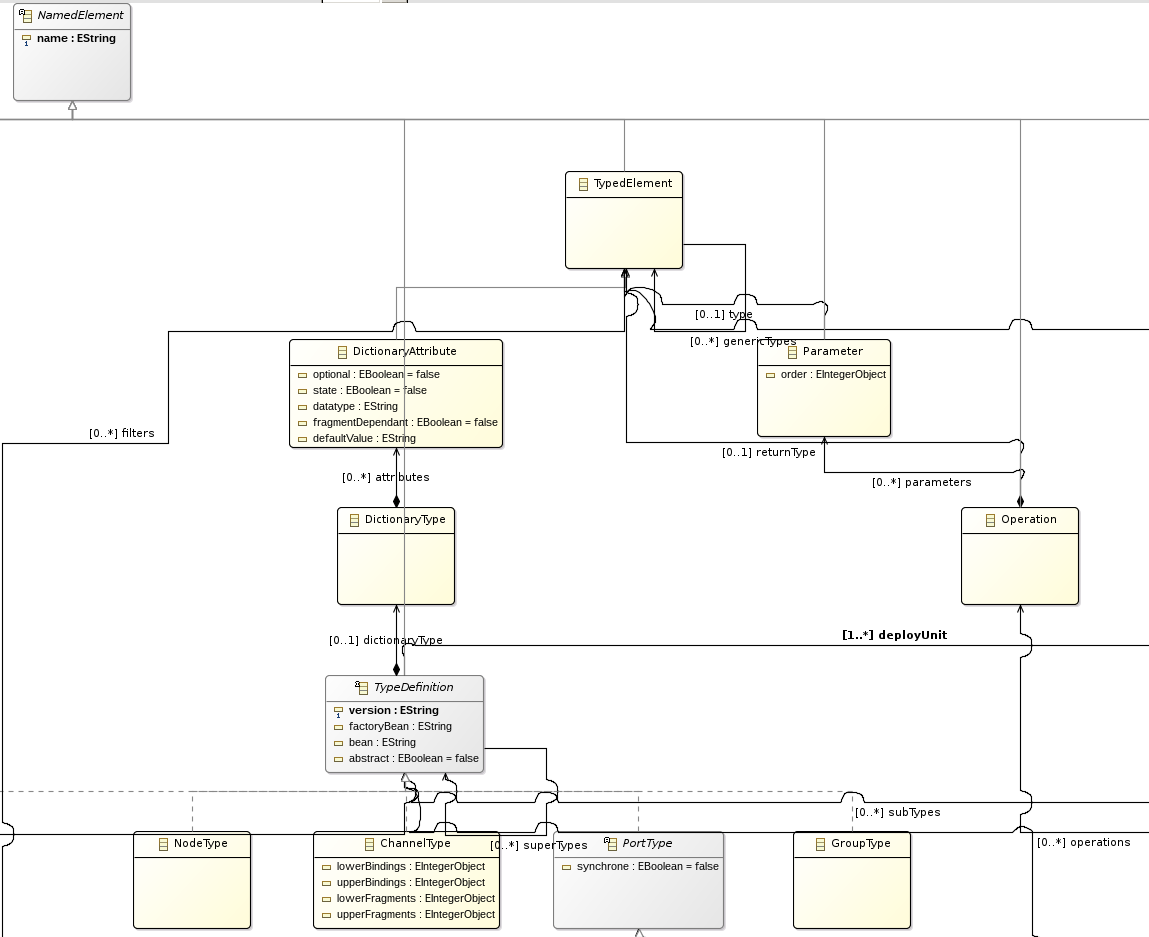
\includegraphics[scale=0.4]{images/kevoree-cd.png}
\caption{Extrait du méta-modèle de Kevoree X écrit en KMF Y}
\label{kevoree-cd}
\end{figure}

\subsection{Structure de \emph{Kevoree}}

Pour résumer \emph{Kevoree-c} est composé d'une structure de données détaillée en section \ref{mm-kevoree}, d'outils de manipulation pour permettre la sérialisation/désérialisation, comparaison de modèles et permettre l'adaptation suite au calcul de ses différences.

\subsection{Résumé du workflow}

% schéma à faire sous inkscape

\subsection{KMFCPP}

l'inspiration, ce qu'il en reste, les limites de leur implém'

\subsection{Une structure de compilateur}

\cite{freeman2004head} \cite{Appel2003MCI599718}

les templates en Velocity Apache,
la représentation interne

\subsection{Générer une structure de données}

Les choix techniques

\subsection{Générer les outils de manipulation}

CMakeLists.txt, fichiers statiques : json.h

serialization, dé-serialization

\section{Avancement, limites et avenir}

Confiance dans le compilateur, les quelques cas ad-hoc




